\documentclass[conference,letterpaper]{IEEEtran}
\usepackage[T1]{fontenc}
\usepackage{array,tabularx}
\usepackage{tikz}
\usetikzlibrary{positioning,arrows.meta}
\usepackage[hidelinks]{hyperref}
\newcolumntype{Y}{>{\raggedright\arraybackslash}X}
\setlength{\tabcolsep}{4pt}
\renewcommand{\arraystretch}{1.12}
\title{VibeGuard: Support Between Therapy Sessions\\Stage 1 Concept and Feasibility Report}
\author{\IEEEauthorblockN{Pina Cammisano}\IEEEauthorblockA{Project I (247-519-VA)\\Vanier College\\November 20, 2026}}
\begin{document}
\maketitle
\begin{abstract}
VibeGuard combines laptop-based facial-expression classification with an ESP32-S3 camera, a voice watch and a WiZ lamp. This Gate 1 report compares concepts, records requirement changes, and assesses technical feasibility, cost and risk. Informal trials demonstrated expression-driven lighting, watch updates and a voice check-in. Counted acceptance testing, reliable camera networking, music integration and spoken correction remain outstanding. The evidence supports requesting progression with conditions; it does not establish therapeutic benefit.
\end{abstract}
\begin{IEEEkeywords}
Facial-expression classification, ESP32-S3, feasibility, embedded systems.
\end{IEEEkeywords}
\section{Changes Since the Proposal}

The October 15 proposal is preserved as the original baseline~\cite{course}.
The current prototype uses a camera-equipped ESP32-S3, an existing
laptop, the required Waveshare watch and a WiZ desk-lamp bulb.

\noindent\textbf{ESP32-C3 to Freenove ESP32-S3 camera kit.} Provides the camera stream and custom controller used in the current prototype.\par

\noindent\textbf{Local laptop classification.} MediaPipe face measurements and personal calibration replace the proposed online facial analysis. Earlier attempts did not establish reliable standalone ESP32 expression recognition.\par

\noindent\textbf{WiZ light bulb and lamp.} Better matches the intended office setting. Current colours are blue for sad, red for mad, white for neutral and gold for happy.\par

\noindent\textbf{REQ-VG-01: automatic decision rule.} Six consecutive winning classified frames replace three readings one minute apart and the neutral approval step. This supports a more responsive demonstration.\par

\noindent\textbf{REQ-VG-03: timing reference.} The five-second response timer begins when a stable label is accepted. The target remains 38 successful trials out of 40.\par

\noindent\textbf{REQ-VG-04: spoken correction.} Moved to future work; conversational replies do not yet override camera labels.\par

\noindent\textbf{REQ-VG-06: hardware budget.} The hardware budget is CAD \$300, including the watch. API expenditure remains separate.\par


\section{Concept Alternatives and Selection}

Three processing approaches were considered while retaining the
watch and custom camera/output hardware. The comparison criteria
were recorded on October 29 before scoring: required behaviour and
performance (30\%), implementation effort (25\%), cost (25\%), and
independence/image handling (20\%). These weights preceded the
current assessment, although an embedded approach was already an
earlier preference.

\noindent\textbf{A: ESP32 inference.} Potential operation without a separate computer; local image processing. Accuracy, model deployment and full hardware operation were not established.\par

\noindent\textbf{B: Remote inference.} Could use a hosted model without local inference hardware. No image service was validated; adds internet, service and usage-cost dependencies.\par

\noindent\textbf{C: Existing laptop.} Runs the current calibrated classifier and coordinates the devices. Requires the laptop to remain available; camera networking still needs improvement.\par

\textbf{Selected concept: C.}\ It has the strongest available integration evidence and uses an
already-owned computer. A remains a possible later development.
B has no demonstrated advantage for this prototype.




\section{Feasibility Case}

The technical objective is to classify four\ \emph{posed facial expressions}\ and produce corresponding device responses.
This does not establish a person's actual feelings or demonstrate
therapeutic benefit. Evidence comes from development records,
manufacturer information and my trials~\cite{records,updates}. Expression trials were not
counted, and controlled acceptance testing remains outstanding.

\begin{figure*}[!t]\centering
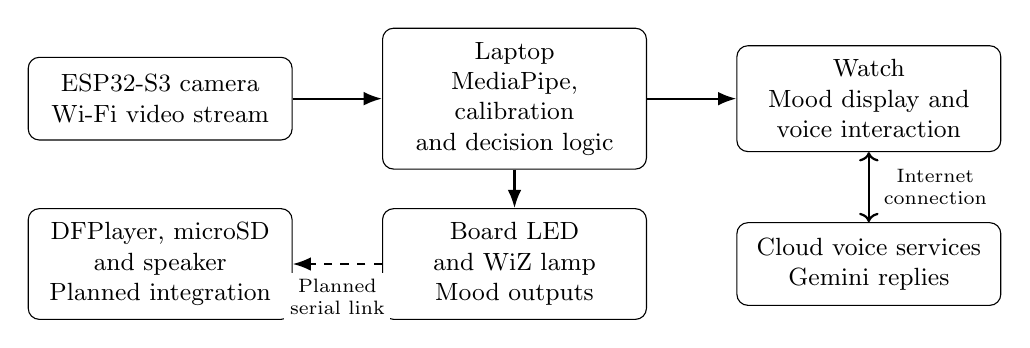
\begin{tikzpicture}[
  box/.style={draw,rounded corners,align=center,
    font=\small,minimum height=1.05cm,text width=3.0cm,
    inner sep=5pt},
  flow/.style={-{Latex},thick},
  planned/.style={-{Latex},thick,dashed},
  linklabel/.style={font=\scriptsize,align=center,
    fill=white,inner sep=2pt}
]
\node[box] (camera) at (0,0)
  {ESP32-S3 camera\\Wi-Fi video stream};
\node[box] (laptop) at (4.5,0)
  {Laptop\\MediaPipe, calibration\\and decision logic};
\node[box] (watch) at (9,0)
  {Watch\\Mood display and\\voice interaction};
\node[box] (music) at (0,-2.1)
  {DFPlayer, microSD\\and speaker\\Planned integration};
\node[box] (outputs) at (4.5,-2.1)
  {Board LED\\and WiZ lamp\\Mood outputs};
\node[box] (cloud) at (9,-2.1)
  {Cloud voice services\\Gemini replies};
\draw[flow] (camera) -- (laptop);
\draw[flow] (laptop) -- (watch);
\draw[flow] (laptop) -- (outputs);
\draw[planned] (outputs.west) --
  node[linklabel,midway,below=3pt]{Planned\\serial link} (music.east);
\draw[flow,<->] (watch.south) --
  node[linklabel,midway,right=3pt]{Internet\\connection} (cloud.north);
\end{tikzpicture}

\caption{Functional diagram. The dashed arrow is the planned serial
connection from the ESP32-S3 controller to the DFPlayer.
The watch sends recordings to Google Gemini over the hotspot's
internet connection.}


\label{fig:system}\end{figure*}

\textbf{Expression classification.}
Initial DeepFace webcam trials ran but frequently confused sad,
mad and neutral expressions. Some faces were not detected.
Later embedded-model investigations did not establish dependable
four-expression recognition.

The working program, \texttt{emotion\_tester.py}, runs on the
laptop. It uses MediaPipe face landmarks and expression
measurements, together with personal calibration, to select happy,
sad, mad or neutral. The calibration is stored in
\texttt{calibration.json}.

I tested the current system on myself and my sister using a single
calibration recorded on my face. All four expressions were classified
correctly in these trials, and the watch and WiZ bulb updated
to match the classified expression. Sad and neutral had previously
been confused before calibration was improved.


\textbf{Camera and network feasibility.}
The ESP32-S3 streams video to the laptop. Reducing image size
previously improved streaming on the phone hotspot.
The devices now connect to a hotspot hosted by the laptop.
With the video stream running, I measured 17 lost test pings out of
20 to the camera board, versus none to the watch and bulb.
This points to the board's Wi-Fi connection rather than a
hotspot-wide failure.

The remaining camera-link issue can interrupt classification.
The proposed fixes require repeat testing. Device addresses can
also change between sessions, so the startup procedure must include
address discovery or reservations.

\textbf{Decision logic and lighting.}
A new mood must win for six consecutive classified frames before
outputs change. The mood is resent every five seconds.
Transitions appeared to occur in under a second during normal
operation, but six frames do not guarantee a fixed time when
streaming slows or drops.

The laptop sends the accepted mood to the board LED, watch and WiZ
bulb. I observed the bulb display blue for sad, red for mad,
white for neutral and gold for happy.




\textbf{Watch and voice feasibility.}
The watch receives and displays the mood. It also performs a
conversational check-in. During a live trial, it asked about sadness;
I replied that I had failed an exam, and the AI responded with
encouragement.

The code triggers a check-in after four seconds of sad or mad,
at most once per minute.

By design, recording runs only while the button is held, up to
eight seconds; this was observed in use. The counted ten-trial
test is still open.
A spoken reply provides context to Gemini but does not change the
camera's label. 

\textbf{Music and electrical integration.}
The DFRobot DFPlayer Mini has been purchased but is not wired or
coded. Manufacturer documentation supports serial control,
microSD playback and direct small-speaker output~\cite{dfplayer}.


The camera kit's 1 GB microSD card will be used in the DFPlayer.
The planned audio circuit uses a 5 V USB supply, a 1 k$\Omega$
serial resistor, a 470 $\mu$F electrolytic capacitor and a
100 nF ceramic capacitor. The DFPlayer will be powered from an
existing USB cable connected to a 5 V supply instead of the
screw-terminal adapter, which would arrive too late. Pin allocation, polarity, common
ground and combined-load behaviour must be checked before testing.
The WiZ bulb receives power through its ordinary lamp connection,
separately from the low-voltage electronics.

\textbf{Cost and buildability.}
My hardware purchases total CAD \$151.32, including the watch
and the full four-speaker pack. This is CAD \$148.68 below the
revised CAD \$300 limit. Allocating only one speaker gives a
parts-used value of CAD \$139.26, but that is not the purchase total.
These costs include tax, with no shipping charges.


I spent CAD \$32 on Gemini API usage; this is an operating cost,
separate from hardware. The BOM and costed work plan are supplied
separately.



\section{Baselined Requirements}
Table~\ref{tab:requirements} records the current acceptance checks and their evidence status. The unmeasured targets remain open.

\begin{table*}[!t]\caption{Baselined requirements and acceptance checks}\label{tab:requirements}\centering\footnotesize
\begin{tabularx}{\linewidth}{|>{\raggedright\arraybackslash}p{1.65cm}|Y|>{\raggedright\arraybackslash}p{2.8cm}|}
\hline
\textbf{ID} & \textbf{Requirement / acceptance check} & \textbf{Status}\\ \hline
REQ-VG-01 &
Six consecutive winning frames permit automatic changes.
Test matching, mixed and interrupted sequences. &
Working in informal trials; formal sequence test pending.\\ \hline
REQ-VG-02 &
At least 28/40 correct posed-expression labels, with per-class results. &
Classification demonstrated; 40-trial target not yet measured.\\ \hline
REQ-VG-03 &
Light and music reach assigned states within five seconds of stable-label
acceptance in at least 38/40 trials. &
Open; music not built.\\ \hline
REQ-VG-04 &
Spoken correction overrides camera labels until the user changes it. &
Unsupported; future work.\\ \hline
REQ-VG-05 &
Record only while talk is held, maximum eight seconds;
verify before, during and after hold in ten trials. &
Partly supported; counted test open.\\ \hline
REQ-VG-06 &
Hardware purchases, including watch, do not exceed CAD \$300. &
Supported by my cost calculation.\\ \hline
REQ-VG-07 &
Controller receives laptop labels wirelessly; watch agrees for all four labels. &
Watch and bulb updates demonstrated; formal consistency test pending.\\ \hline
REQ-VG-08 &
Build and run from a clean GitHub copy using written steps on another computer. &
Open; independent rebuild pending.\\ \hline
\end{tabularx}
\end{table*}



\section{Updated Risk Register}

The following is a provisional engineering assessment.
Probability (P) and consequence (C) use 1 = low, 2 = medium,
3 = high. Priority is $P \times C$, with ties ranked by higher
consequence. These scores are judgments, not measured probabilities. Table~\ref{tab:risks} records the evidence required and mitigations.

\begin{table*}[!t]\caption{Updated risk register}\label{tab:risks}\centering\footnotesize
\begin{tabularx}{\linewidth}{|>{\raggedright\arraybackslash}p{0.22\linewidth}|Y|c|c|c|Y|}
\hline
\textbf{Risk / assumption} &
\textbf{Consequence} &
\textbf{P} & \textbf{C} & \textbf{Priority} &
\textbf{Evidence required and mitigation}\\ \hline
Camera link drops; assumes hotspot sustains video &
Classification stalls or outputs become stale. &
3&3&9&
Log video/link behaviour after restart; test reduced stream load
and stale-data handling.\\ \hline
Calibration does not generalize; assumes poses remain separable &
Incorrect classification and environment response. &
2&3&6&
Run counted trials with calibration conditions stated;
record per-class errors and implement correction.\\ \hline
DFPlayer integration fails; assumes available pins and power suffice &
Music requirement remains untested. &
3&2&6&
Verify pin/power plan; test playback alone and with camera active.\\ \hline
Voice credentials or service limits interrupt replies &
Voice interaction unavailable. &
2&2&4&
Repeat held-button trials; document credentials, billing limits
and failure recovery.\\ \hline
Device addresses change; assumes endpoints stay valid &
Manual startup fails after restart. &
2&2&4&
Run fresh-start test; document address discovery or reservations.\\ \hline
Spoken override remains unfinished &
User cannot correct a persistent wrong label. &
2&2&4&
Demonstrate correction persists through later camera updates;
retain as explicit implementation milestone.\\ \hline
\end{tabularx}
\end{table*}

\begin{center}
\begin{tabularx}{\columnwidth}{|l|c|Y|Y|}
\hline
& \textbf{C1} & \textbf{C2} & \textbf{C3}\\ \hline
\textbf{P3: High} & --- & Music integration & Camera link\\ \hline
\textbf{P2: Medium} & --- & Voice, addresses, spoken override &
Classification\\ \hline
\textbf{P1: Low} & --- & --- & ---\\ \hline
\end{tabularx}
\end{center}

The principal risks have shifted from uncertain component selection
toward camera reliability, classification evidence and unfinished
integration. Hardware cost is now better established, while the
full prototype completion date remains unknown.

\section{Gate 1 Readiness}

The current evidence supports requesting progression
\textbf{with conditions}. I demonstrated camera, watch and lighting
integration and a conversational check-in. My hardware purchases
are within the revised budget.
The required watch and meaningful custom hardware remain in scope.

The next work is to:
\begin{itemize}
\item stabilize camera streaming and document repeatable startup;
\item wire and program the DFPlayer music subsystem;
\item record the 40 expression trials, 40 response-time trials
and ten hold-to-talk trials;
\item implement persistent spoken correction;
\item verify a clean-copy build on another computer.
\end{itemize}

\begin{samepage}
The separate costed work plan identifies dependencies and estimated
effort. Gate 1 is due November 20, 2026; the final prototype deadline
must still be confirmed. Remaining work is disclosed rather than
presented as completed. The instructor determines the actual gate outcome.
\end{samepage}



\begin{thebibliography}{4}
\bibitem{course} Course handout,
\emph{Part B: Writing the Stage 1 Concept and Feasibility Report};
and frozen \emph{Vibe Guard} proposal, revised October 15, 2026.
\bibitem{dfplayer} DFRobot, \emph{DFPlayer Mini, DFR0299}.
\url{https://wiki.dfrobot.com/dfr0299}.
Consulted November 2026.
\bibitem{records} VibeGuard project logbook and research references,
October 23--November 18, 2026: model investigations, component
selection, integration observations and report baseline.
\bibitem{updates} Student report updates, November 18, 2026:
shared calibration trial, live watch check-in,
bulb colours, current limitations and itemized costs.
\end{thebibliography}

\end{document}

